\section{Ejercicio 3: Medici\'on de un glitch}

El prop\'osito de este apartado es analizar el comportamiento de un circuito l\'ogico determinado, implementado con compuertas f\'isicas. Dicho circuito corresponde a la tabla de verdad que se reproduce a continuaci\'on.

\begin{table}[H]
\centering
\label{tab:ej3_tabla_verdad}
\begin{tabular}{ccc|c}
A & B & C & Y \\ \hline
0 & 0 & 0 & 0 \\
0 & 0 & 1 & 1 \\
0 & 1 & 0 & 1 \\
0 & 1 & 1 & 1 \\
1 & 0 & 0 & 0 \\
1 & 0 & 1 & 1 \\
1 & 1 & 0 & 0 \\
1 & 1 & 1 & 0
\end{tabular}
\caption{Tabla de verdad}
\end{table}

\subsection{S\'intesis del circuito}
Para lograr el equivalente circuital de la tabla anterior se emplea un mapa de Karnaugh, de forma tal de lograr la expresi\'on m\'as simplificada, y por ende la de menor costo.

\begin{center}
    \begin{Karnaughvuit}
        \label{Karnaugh_glitch}
        \contingut{0,1,2,3,4,5,6,7}
        \implicant{3}{2}{green}
        \implicant{1}{5}{green}
	\end{Karnaughvuit}\\
Mapa de Karnaugh
\end{center}


Agrupando en mint\'erminos a los grupos resaltados en el mapa se llega a la siguiente expresi\'on:

\begin{equation}
\label{ej3_glitheq}
 Y = \overline{A}\cdot B + C \cdot \overline{B}
\end{equation}

En teor\'ia, el circuito resultante de \ref{ej3_glitheq} deber\'ia responder exactamente a la tabla de verdad. Observando el mapa de Karnaugh se puede concluir que existe la posibilidad de que suceda un glitch en la transici\'on del estado $(A = 0, B = 0, C = 1)$ al estado $(A = 0, B = 1, C = 1)$ (gr\'aficamente esto puede ser apreciado en la adyacencia existente entre los dos grupos). Es decir, es posible que la salida del circuito se comporte de forma inesperada, presentando por un instante un cero l\'ogico. Esta situaci\'on puede ser riesgosa si se tratara de un circuito l\'ogico real operando en su entorno de trabajo, dado que se podr\'ian desencadenar acciones indeseadas por parte de la etapa cuya entrada es el circuito que se analiza.

Para prevenir esto, se puede agregar un grupo extra que contenga las posiciones cuya transici\'on pudiera ser conflictiva. Si se implementa lo anterior se obtiene el siguiente mapa de karnaugh, con su correspondiente expresi\'on l\'ogica asociada.

\begin{center}

    \begin{Karnaughvuit}
        \label{Karnaugh_noglitch}
        \contingut{0,1,2,3,4,5,6,7}
        \implicant{3}{2}{green}
        \implicant{1}{5}{green}
        \implicant{1}{3}{blue}
\end{Karnaughvuit}\\
Mapa de Karnaugh correcci\'on de glitch
\end{center}

Los grupos que componen la soluci\'on de menor costo est\'an simbolizados en color verde, mientras que el grupo auxiliar est\'a marcado en azul.

\begin{equation}
\label{ej3_noglitheq}
 Y = \overline{A}\cdot B + C \cdot \overline{B} + \overline{A} \cdot C
\end{equation}

De esta forma, se asegura que la transici\'on entre las posiciones en conflicto sea la esperada, corrigiendo el problema. Como se puede observar, la ecuaci\'on~\ref{ej3_noglitheq} es la expresi\'on~\ref{ej3_glitheq} sumando al t\'ermino $\overline{A} \cdot C$. Se obtiene el circuito l\'ogico que se reproduce a continuaci\'on, resaltando en color verde las compuertas agregadas para implementar la correcci\'on.

\begin{figure}[H]
    \centering
    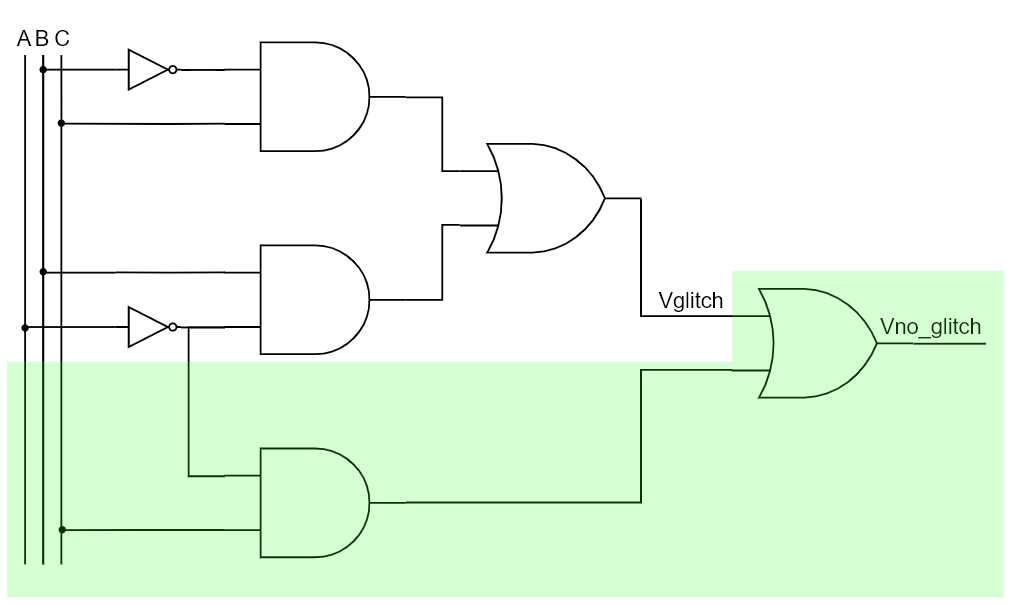
\includegraphics[width=0.9\textwidth]{../EJ3/Recursos/EJ3_logic_circuit}
	\caption{Circuito l\'ogico}
   	\label{fig:EJ3_logic_circuit}
\end{figure}

\subsection{Implementaci\'on y medici\'on del circuito}

Se arm\'o el circuito de la figura~\ref{fig:EJ3_logic_circuit} utilizando los siguientes integrados para cada tipo de compuerta l\'ogica.

\begin{table}[H]
    \centering
    \begin{tabular}{c c}
        Compuerta & Circuito integrado\\
        \hline
        $AND$ & $74HC08$ \\
        $OR$ & $74HC32$\\
        $NOT$ & $74HC04$\\
        \hline
    \end{tabular}
    \caption{IC empleados en implementaci\'on}
\end{table}

Se establecieron las condiciones de las entradas de tal forma de solo variar la variable \textsc{"B"}, emulando el cambio con una se\~nal cuadrada que oscila entre $0V$ y $5V$ a una frecuencia de $30kHz$. En primera instancia se observ\'o detalladamente el comportamiento de ambas salidas del circuito (con mint\'ermino de correcci\'on y sin el mismo) cuando el flanco de la se\~nal de entrada es ascendente. Se observan las siguientes respuestas (siendo la se\~nal de entrada color violeta, la se\~nal sin correcci\'on amarilla y la se\~nal con correcci\'on verde).

\begin{figure}[H]
    \centering
    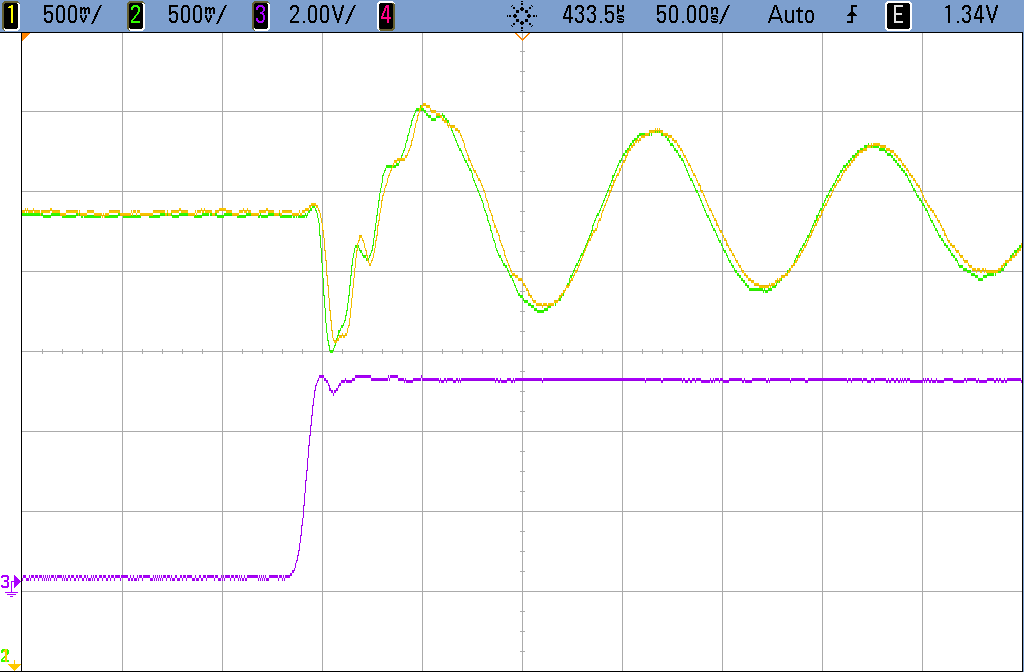
\includegraphics[width=0.9\textwidth]{../EJ3/Recursos/cropped_EJ3_positive_slope_response.png}
	\caption{Respuesta del circuito en flanco ascendente}
   	\label{fig:EJ3_positive_slope_response}
\end{figure}

En la figura anterior se puede apreciar una respuesta oscilatoria subamortiguada del circuito, destacando que ambas salidas presentan exactamente la misma oscilaci\'on. Se observa que en sus picos m\'aximos, las se\~nales de salida var\'ian entre $4V$ y $5.5V$. Estos niveles de tensi\'on se encuentran dentro del rango HIGH de una compuerta CMOS y de una del tipo TTL. De esta manera, no se puede considerar que exista un glitch en ninguna de las salidas.

An\'alogamente, se repiti\'o la medici\'on para un flanco descendente, reflejando los siguientes resultados (con la combinaci\'on de colores antes mencionada).

\begin{figure}[H]
    \centering
    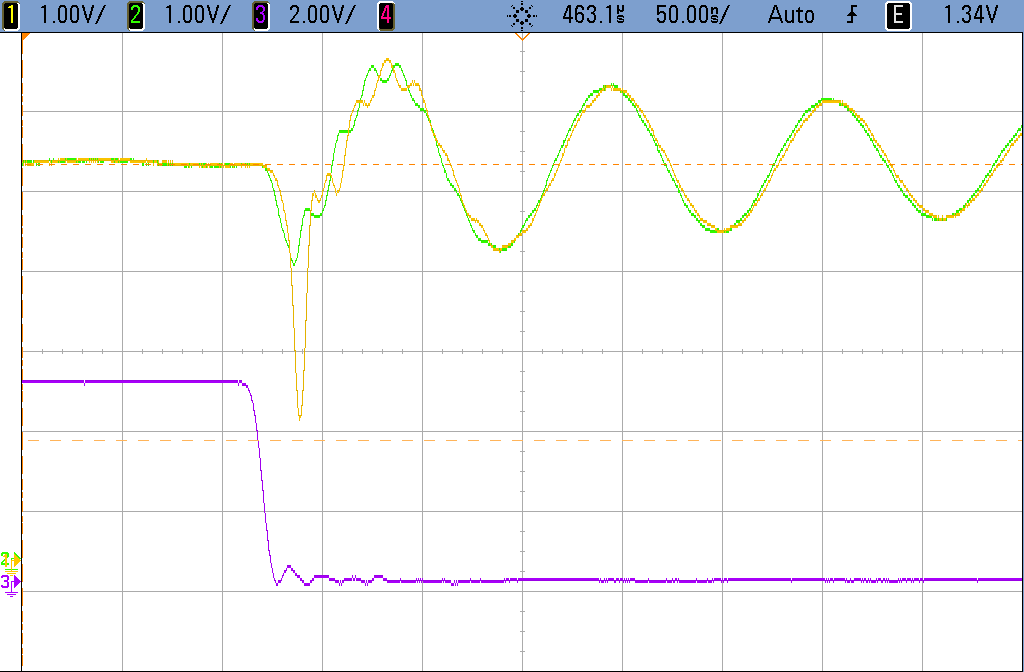
\includegraphics[width=0.9\textwidth]{../EJ3/Recursos/cropped_EJ3_negative_slope_response.png}
	\caption{Respuesta del circuito en flanco descendente}
   	\label{fig:EJ3_negative_slope_response}
\end{figure}

Para este caso s\'i se aprecia una diferencia razonable entre ambas respuestas: mientras que la oscilaci\'on de la salida compensada esta comprendida en un rango que va desde $3,8V$ hasta $5,8V$ (ambas dentro de los l\'imites aceptables de HIGH en ambas tecnolog\'ias), el l\'imite inferior del sobrepico de la salida sin compensar se acerca a $2,5V$. Este \'ultimo valor de tensi\'on se ubica por debajo de los rangos normales de entrada en HIGH, por lo que podr\'ia ser intepretada como un cero l\'ogico por el circuito cuya entrada es la salida de este. Asimismo, cabe destacar que el per\'iodo de duraci\'on del glitch es cercano a los $100 \mu s$, que es un tiempo relativamente corto. De todas formas, el impacto del glitch depender\'a de las caracter\'isticas del ciruito que reciba la se\~nal de salida de este. 

Este fen\'omeno se produce debido al tiempo de propagaci\'on de las entradas a trav\'es de las sucesivas etapas compuestas por compuertas l\'ogicas. Especialmente debido a que el camino circuital que recorren las se\~nales no les insume el mismo tiempo,  dado que es probable que una se\~nal determinada deba propagarse por m\'as compuertas que otras, gener\'andose una condici\'on de asimetr\'ia en el procesamiento. 

Por \'ultimo, se advierte que el tiempo en el que se estabiliza la oscilaci\'on es cercano a los $2,35ns$ como se aprecia en imagen de abajo.

\begin{figure}[H]
    \centering
    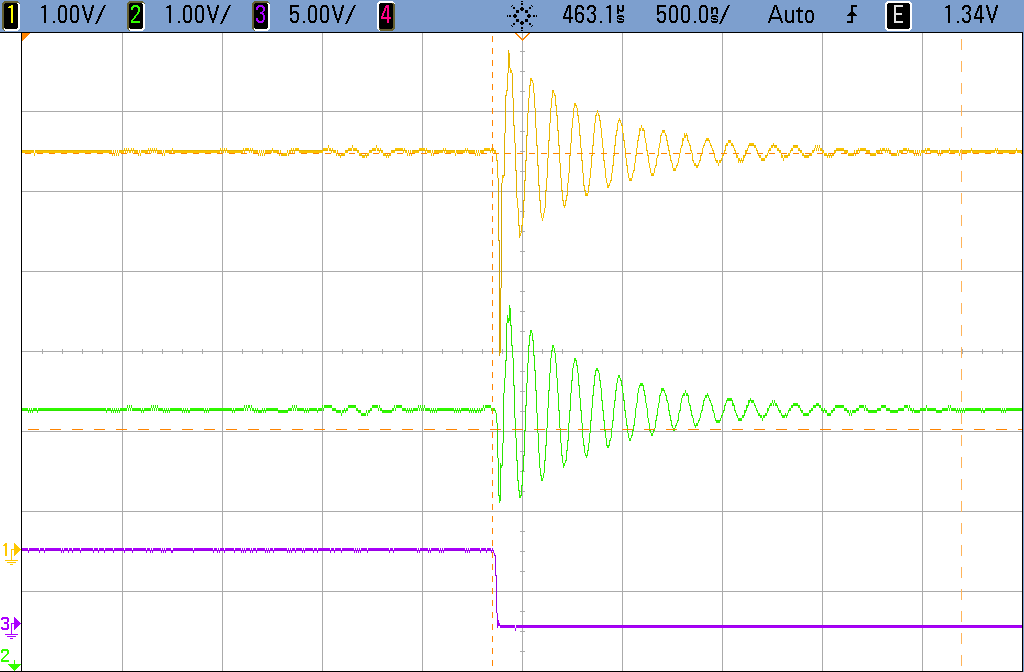
\includegraphics[width=0.9\textwidth]{../EJ3/Recursos/cropped_EJ3_negative_slope_response_zout.png}
	\caption{Respuesta del circuito en flanco descendente - Establecimiento}
   	\label{fig:EJ3_negative_slope_response_zout}
\end{figure}

\subsection{Conclusi\'on}
Como conclusi\'on, se puede destacar que el circuito sin compensar no ser\'ia seguro de implementar en una aplicaci\'on que requiera una alta confiabilidad del circuito. Dependiendo de la aplicaci\'on y del nivel de confiabilidad deseado se debe tener en cuenta el agregado del mint\'ermino de compensaci\'on, como se pudo observar con anterioridad.





